\documentclass{standalone}
\usepackage{tikz}
\usetikzlibrary{patterns, positioning}


\begin{document}
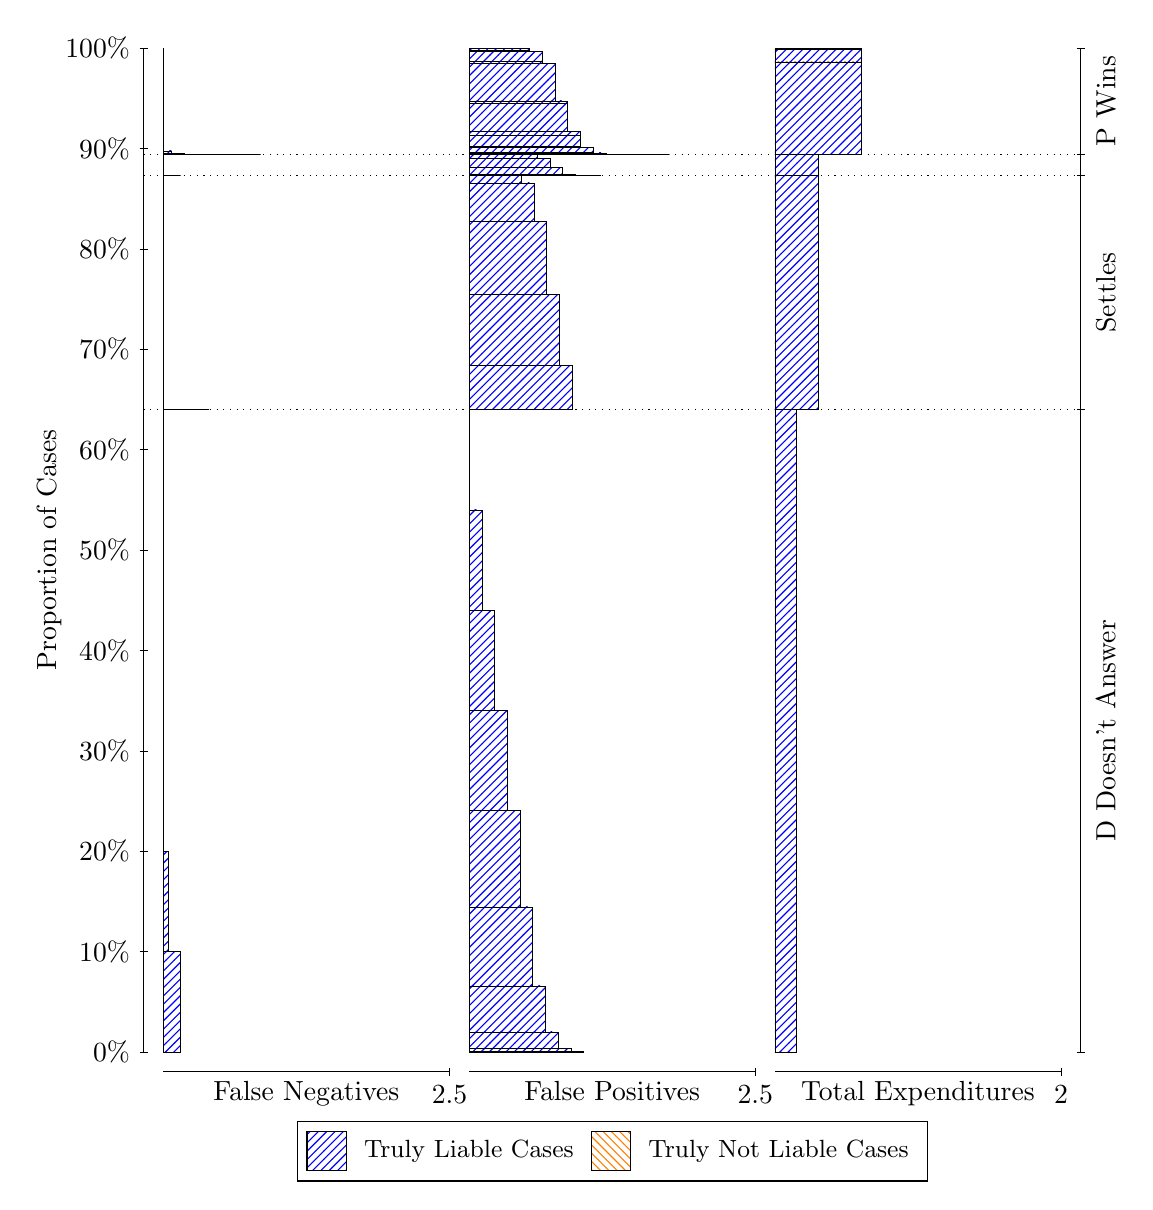
\begin{tikzpicture}
\draw[black, very thin] (1.5,1.75) -- (1.5,14.5);
\node[rotate=90, text=black, anchor=center] at (0.3, 8.125) {Proportion of Cases};
\draw[black, very thin] (1.45,1.75) -- (1.55,1.75);
\node[text=black, anchor=east] at (1.45, 1.75) {0\%};
\draw[black, very thin] (1.45,3.025) -- (1.55,3.025);
\node[text=black, anchor=east] at (1.45, 3.025) {10\%};
\draw[black, very thin] (1.45,4.3) -- (1.55,4.3);
\node[text=black, anchor=east] at (1.45, 4.3) {20\%};
\draw[black, very thin] (1.45,5.575) -- (1.55,5.575);
\node[text=black, anchor=east] at (1.45, 5.575) {30\%};
\draw[black, very thin] (1.45,6.85) -- (1.55,6.85);
\node[text=black, anchor=east] at (1.45, 6.85) {40\%};
\draw[black, very thin] (1.45,8.125) -- (1.55,8.125);
\node[text=black, anchor=east] at (1.45, 8.125) {50\%};
\draw[black, very thin] (1.45,9.4) -- (1.55,9.4);
\node[text=black, anchor=east] at (1.45, 9.4) {60\%};
\draw[black, very thin] (1.45,10.675) -- (1.55,10.675);
\node[text=black, anchor=east] at (1.45, 10.675) {70\%};
\draw[black, very thin] (1.45,11.95) -- (1.55,11.95);
\node[text=black, anchor=east] at (1.45, 11.95) {80\%};
\draw[black, very thin] (1.45,13.225) -- (1.55,13.225);
\node[text=black, anchor=east] at (1.45, 13.225) {90\%};
\draw[black, very thin] (1.45,14.5) -- (1.55,14.5);
\node[text=black, anchor=east] at (1.45, 14.5) {100\%};

\draw[black, very thin] (13.4,1.75) -- (13.4,14.5);
\draw[black, very thin] (13.35,1.75) -- (13.45,1.75);
\node[anchor=west] at (13.35, 1.75) {};
\draw[black, very thin] (13.35,9.909) -- (13.45,9.909);
\node[anchor=west] at (13.35, 9.909) {};
\draw[black, very thin] (13.35,12.885) -- (13.45,12.885);
\node[anchor=west] at (13.35, 12.885) {};
\draw[black, very thin] (13.35,13.15) -- (13.45,13.15);
\node[anchor=west] at (13.35, 13.15) {};
\draw[black, very thin] (13.35,14.5) -- (13.45,14.5);
\node[anchor=west] at (13.35, 14.5) {};

\draw[black, very thin, pattern color=blue, pattern=north east lines] (1.75,1.75) rectangle (1.968,3.025);
\draw[black, very thin, pattern color=blue, pattern=north east lines] (1.75,3.025) rectangle (1.8065,4.3);
\draw[black, very thin, pattern color=orange, pattern=north west lines] (1.75,4.3) rectangle (1.75,4.3);
\draw[black, very thin, pattern color=blue, pattern=north east lines] (1.75,4.3) rectangle (1.75,9.909);
\draw[black, very thin, pattern color=blue, pattern=north east lines] (1.75,9.909) rectangle (2.3313,9.909);
\draw[black, very thin, pattern color=blue, pattern=north east lines] (1.75,9.909) rectangle (2.1699,9.909);
\draw[black, very thin, pattern color=blue, pattern=north east lines] (1.75,9.909) rectangle (2.0084,9.909);
\draw[black, very thin, pattern color=blue, pattern=north east lines] (1.75,9.909) rectangle (1.8469,9.9091);
\draw[black, very thin, pattern color=orange, pattern=north west lines] (1.75,9.9091) rectangle (1.75,9.9091);
\draw[black, very thin, pattern color=blue, pattern=north east lines] (1.75,9.9091) rectangle (1.75,12.885);
\draw[black, very thin, pattern color=blue, pattern=north east lines] (1.75,12.885) rectangle (1.968,12.885);
\draw[black, very thin, pattern color=blue, pattern=north east lines] (1.75,12.885) rectangle (1.8065,12.885);
\draw[black, very thin, pattern color=orange, pattern=north west lines] (1.75,12.885) rectangle (1.75,12.885);
\draw[black, very thin, pattern color=blue, pattern=north east lines] (1.75,12.885) rectangle (1.75,13.15);
\draw[black, very thin, pattern color=blue, pattern=north east lines] (1.75,13.15) rectangle (2.9853,13.15);
\draw[black, very thin, pattern color=blue, pattern=north east lines] (1.75,13.15) rectangle (2.8239,13.15);
\draw[black, very thin, pattern color=blue, pattern=north east lines] (1.75,13.15) rectangle (2.6624,13.15);
\draw[black, very thin, pattern color=blue, pattern=north east lines] (1.75,13.15) rectangle (2.5009,13.15);
\draw[black, very thin, pattern color=blue, pattern=north east lines] (1.75,13.15) rectangle (2.5009,13.15);
\draw[black, very thin, pattern color=blue, pattern=north east lines] (1.75,13.15) rectangle (2.3394,13.15);
\draw[black, very thin, pattern color=blue, pattern=north east lines] (1.75,13.15) rectangle (2.3394,13.15);
\draw[black, very thin, pattern color=blue, pattern=north east lines] (1.75,13.15) rectangle (2.3394,13.15);
\draw[black, very thin, pattern color=blue, pattern=north east lines] (1.75,13.15) rectangle (2.1779,13.15);
\draw[black, very thin, pattern color=blue, pattern=north east lines] (1.75,13.15) rectangle (2.1779,13.151);
\draw[black, very thin, pattern color=blue, pattern=north east lines] (1.75,13.151) rectangle (2.0164,13.151);
\draw[black, very thin, pattern color=blue, pattern=north east lines] (1.75,13.151) rectangle (2.0164,13.151);
\draw[black, very thin, pattern color=blue, pattern=north east lines] (1.75,13.151) rectangle (2.0164,13.158);
\draw[black, very thin, pattern color=blue, pattern=north east lines] (1.75,13.158) rectangle (1.855,13.159);
\draw[black, very thin, pattern color=blue, pattern=north east lines] (1.75,13.159) rectangle (1.855,13.193);
\draw[black, very thin, pattern color=blue, pattern=north east lines] (1.75,13.193) rectangle (1.855,13.193);
\draw[black, very thin, pattern color=orange, pattern=north west lines] (1.75,13.193) rectangle (1.75,13.193);
\draw[black, very thin, pattern color=blue, pattern=north east lines] (1.75,13.193) rectangle (1.75,14.5);
\draw[black, very thin, pattern color=orange, pattern=north west lines] (5.6333,1.75) rectangle (7.0867,1.75);
\draw[black, very thin, pattern color=blue, pattern=north east lines] (5.6333,1.75) rectangle (7.0867,1.7548);
\draw[black, very thin, pattern color=blue, pattern=north east lines] (5.6333,1.7548) rectangle (6.9252,1.796);
\draw[black, very thin, pattern color=blue, pattern=north east lines] (5.6333,1.796) rectangle (6.7637,2.0041);
\draw[black, very thin, pattern color=blue, pattern=north east lines] (5.6333,2.0041) rectangle (6.6022,2.5904);
\draw[black, very thin, pattern color=blue, pattern=north east lines] (5.6333,2.5904) rectangle (6.4407,3.5938);
\draw[black, very thin, pattern color=blue, pattern=north east lines] (5.6333,3.5938) rectangle (6.2793,4.8141);
\draw[black, very thin, pattern color=blue, pattern=north east lines] (5.6333,4.8141) rectangle (6.1178,6.0842);
\draw[black, very thin, pattern color=blue, pattern=north east lines] (5.6333,6.0842) rectangle (5.9563,7.359);
\draw[black, very thin, pattern color=blue, pattern=north east lines] (5.6333,7.359) rectangle (5.7948,8.634);
\draw[black, very thin, pattern color=blue, pattern=north east lines] (5.6333,8.634) rectangle (5.6333,9.909);
\draw[black, very thin, pattern color=orange, pattern=north west lines] (5.6333,9.909) rectangle (6.9413,9.909);
\draw[black, very thin, pattern color=blue, pattern=north east lines] (5.6333,9.909) rectangle (6.9413,10.473);
\draw[black, very thin, pattern color=blue, pattern=north east lines] (5.6333,10.473) rectangle (6.7799,11.371);
\draw[black, very thin, pattern color=blue, pattern=north east lines] (5.6333,11.371) rectangle (6.6184,12.299);
\draw[black, very thin, pattern color=blue, pattern=north east lines] (5.6333,12.299) rectangle (6.4569,12.786);
\draw[black, very thin, pattern color=blue, pattern=north east lines] (5.6333,12.786) rectangle (6.2954,12.88);
\draw[black, very thin, pattern color=blue, pattern=north east lines] (5.6333,12.88) rectangle (6.1339,12.885);
\draw[black, very thin, pattern color=blue, pattern=north east lines] (5.6333,12.885) rectangle (5.9724,12.885);
\draw[black, very thin, pattern color=blue, pattern=north east lines] (5.6333,12.885) rectangle (5.811,12.885);
\draw[black, very thin, pattern color=blue, pattern=north east lines] (5.6333,12.885) rectangle (5.6495,12.885);
\draw[black, very thin, pattern color=blue, pattern=north east lines] (5.6333,12.885) rectangle (5.6333,12.885);
\draw[black, very thin, pattern color=orange, pattern=north west lines] (5.6333,12.885) rectangle (7.3047,12.885);
\draw[black, very thin, pattern color=blue, pattern=north east lines] (5.6333,12.885) rectangle (7.3047,12.885);
\draw[black, very thin, pattern color=blue, pattern=north east lines] (5.6333,12.885) rectangle (7.1432,12.885);
\draw[black, very thin, pattern color=blue, pattern=north east lines] (5.6333,12.885) rectangle (6.9817,12.897);
\draw[black, very thin, pattern color=blue, pattern=north east lines] (5.6333,12.897) rectangle (6.8202,12.981);
\draw[black, very thin, pattern color=blue, pattern=north east lines] (5.6333,12.981) rectangle (6.6587,13.103);
\draw[black, very thin, pattern color=blue, pattern=north east lines] (5.6333,13.103) rectangle (6.4973,13.146);
\draw[black, very thin, pattern color=blue, pattern=north east lines] (5.6333,13.146) rectangle (6.3358,13.15);
\draw[black, very thin, pattern color=blue, pattern=north east lines] (5.6333,13.15) rectangle (6.1743,13.15);
\draw[black, very thin, pattern color=blue, pattern=north east lines] (5.6333,13.15) rectangle (6.0128,13.15);
\draw[black, very thin, pattern color=blue, pattern=north east lines] (5.6333,13.15) rectangle (5.8513,13.15);
\draw[black, very thin, pattern color=orange, pattern=north west lines] (5.6333,13.15) rectangle (8.1767,13.15);
\draw[black, very thin, pattern color=blue, pattern=north east lines] (5.6333,13.15) rectangle (8.1767,13.15);
\draw[black, very thin, pattern color=orange, pattern=north west lines] (5.6333,13.15) rectangle (8.0152,13.15);
\draw[black, very thin, pattern color=blue, pattern=north east lines] (5.6333,13.15) rectangle (8.0152,13.15);
\draw[black, very thin, pattern color=orange, pattern=north west lines] (5.6333,13.15) rectangle (7.8537,13.15);
\draw[black, very thin, pattern color=blue, pattern=north east lines] (5.6333,13.15) rectangle (7.8537,13.15);
\draw[black, very thin, pattern color=blue, pattern=north east lines] (5.6333,13.15) rectangle (7.6922,13.15);
\draw[black, very thin, pattern color=orange, pattern=north west lines] (5.6333,13.15) rectangle (7.6922,13.15);
\draw[black, very thin, pattern color=blue, pattern=north east lines] (5.6333,13.15) rectangle (7.6922,13.151);
\draw[black, very thin, pattern color=orange, pattern=north west lines] (5.6333,13.151) rectangle (7.5307,13.151);
\draw[black, very thin, pattern color=blue, pattern=north east lines] (5.6333,13.151) rectangle (7.5307,13.152);
\draw[black, very thin, pattern color=blue, pattern=north east lines] (5.6333,13.152) rectangle (7.5307,13.153);
\draw[black, very thin, pattern color=orange, pattern=north west lines] (5.6333,13.153) rectangle (7.3693,13.153);
\draw[black, very thin, pattern color=blue, pattern=north east lines] (5.6333,13.153) rectangle (7.3693,13.167);
\draw[black, very thin, pattern color=blue, pattern=north east lines] (5.6333,13.167) rectangle (7.3693,13.168);
\draw[black, very thin, pattern color=blue, pattern=north east lines] (5.6333,13.168) rectangle (7.2078,13.173);
\draw[black, very thin, pattern color=orange, pattern=north west lines] (5.6333,13.173) rectangle (7.2078,13.173);
\draw[black, very thin, pattern color=blue, pattern=north east lines] (5.6333,13.173) rectangle (7.2078,13.238);
\draw[black, very thin, pattern color=blue, pattern=north east lines] (5.6333,13.238) rectangle (7.0463,13.251);
\draw[black, very thin, pattern color=orange, pattern=north west lines] (5.6333,13.251) rectangle (7.0463,13.251);
\draw[black, very thin, pattern color=blue, pattern=north east lines] (5.6333,13.251) rectangle (7.0463,13.39);
\draw[black, very thin, pattern color=blue, pattern=north east lines] (5.6333,13.39) rectangle (7.0463,13.441);
\draw[black, very thin, pattern color=orange, pattern=north west lines] (5.6333,13.441) rectangle (6.8848,13.441);
\draw[black, very thin, pattern color=blue, pattern=north east lines] (5.6333,13.441) rectangle (6.8848,13.798);
\draw[black, very thin, pattern color=blue, pattern=north east lines] (5.6333,13.798) rectangle (6.8848,13.827);
\draw[black, very thin, pattern color=blue, pattern=north east lines] (5.6333,13.827) rectangle (6.8848,13.828);
\draw[black, very thin, pattern color=orange, pattern=north west lines] (5.6333,13.828) rectangle (6.7233,13.828);
\draw[black, very thin, pattern color=blue, pattern=north east lines] (5.6333,13.828) rectangle (6.7233,14.307);
\draw[black, very thin, pattern color=blue, pattern=north east lines] (5.6333,14.307) rectangle (6.7233,14.307);
\draw[black, very thin, pattern color=blue, pattern=north east lines] (5.6333,14.307) rectangle (6.5619,14.335);
\draw[black, very thin, pattern color=blue, pattern=north east lines] (5.6333,14.335) rectangle (6.5619,14.458);
\draw[black, very thin, pattern color=blue, pattern=north east lines] (5.6333,14.458) rectangle (6.5619,14.458);
\draw[black, very thin, pattern color=blue, pattern=north east lines] (5.6333,14.458) rectangle (6.4004,14.471);
\draw[black, very thin, pattern color=blue, pattern=north east lines] (5.6333,14.471) rectangle (6.4004,14.492);
\draw[black, very thin, pattern color=blue, pattern=north east lines] (5.6333,14.492) rectangle (6.4004,14.493);
\draw[black, very thin, pattern color=blue, pattern=north east lines] (5.6333,14.493) rectangle (6.2389,14.495);
\draw[black, very thin, pattern color=blue, pattern=north east lines] (5.6333,14.495) rectangle (6.2389,14.499);
\draw[black, very thin, pattern color=blue, pattern=north east lines] (5.6333,14.499) rectangle (6.2389,14.499);
\draw[black, very thin, pattern color=blue, pattern=north east lines] (5.6333,14.499) rectangle (6.2389,14.499);
\draw[black, very thin, pattern color=blue, pattern=north east lines] (5.6333,14.499) rectangle (6.0774,14.5);
\draw[black, very thin, pattern color=blue, pattern=north east lines] (5.6333,14.5) rectangle (6.0774,14.5);
\draw[black, very thin, pattern color=blue, pattern=north east lines] (5.6333,14.5) rectangle (5.9159,14.5);
\draw[black, very thin, pattern color=blue, pattern=north east lines] (5.6333,14.5) rectangle (5.9159,14.5);
\draw[black, very thin, pattern color=blue, pattern=north east lines] (5.6333,14.5) rectangle (5.7544,14.5);
\draw[black, very thin, pattern color=blue, pattern=north east lines] (5.6333,14.5) rectangle (5.7544,14.5);
\draw[black, very thin, pattern color=blue, pattern=north east lines] (5.6333,14.5) rectangle (5.6333,14.5);
\draw[black, very thin, pattern color=orange, pattern=north west lines] (9.5167,1.75) rectangle (9.7892,1.75);
\draw[black, very thin, pattern color=blue, pattern=north east lines] (9.5167,1.75) rectangle (9.7892,9.909);
\draw[black, very thin, pattern color=orange, pattern=north west lines] (9.5167,9.909) rectangle (10.062,9.909);
\draw[black, very thin, pattern color=blue, pattern=north east lines] (9.5167,9.909) rectangle (10.062,12.885);
\draw[black, very thin, pattern color=orange, pattern=north west lines] (9.5167,12.885) rectangle (10.062,12.885);
\draw[black, very thin, pattern color=blue, pattern=north east lines] (9.5167,12.885) rectangle (10.062,13.15);
\draw[black, very thin, pattern color=orange, pattern=north west lines] (9.5167,13.15) rectangle (10.607,13.15);
\draw[black, very thin, pattern color=blue, pattern=north east lines] (9.5167,13.15) rectangle (10.607,14.323);
\draw[black, very thin, pattern color=orange, pattern=north west lines] (9.5167,14.323) rectangle (10.607,14.323);
\draw[black, very thin, pattern color=blue, pattern=north east lines] (9.5167,14.323) rectangle (10.607,14.482);
\draw[black, very thin, pattern color=orange, pattern=north west lines] (9.5167,14.482) rectangle (10.607,14.482);
\draw[black, very thin, pattern color=blue, pattern=north east lines] (9.5167,14.482) rectangle (10.607,14.5);
\draw[black, dotted] (1.5,9.909) -- (13.4,9.909);
\draw[black, dotted] (1.5,12.885) -- (13.4,12.885);
\draw[black, dotted] (1.5,13.15) -- (13.4,13.15);
\draw[black, very thin] (1.75,1.5) -- (5.3833,1.5);
\node[text=black, anchor=north] at (3.5667, 1.5) {False Negatives};
\draw[black, very thin] (5.3833,1.45) -- (5.3833,1.55);
\node[text=black, anchor=north] at (5.3833, 1.45) {2.5};

\draw[black, very thin] (5.6333,1.5) -- (9.2667,1.5);
\node[text=black, anchor=north] at (7.45, 1.5) {False Positives};
\draw[black, very thin] (9.2667,1.45) -- (9.2667,1.55);
\node[text=black, anchor=north] at (9.2667, 1.45) {2.5};

\draw[black, very thin] (9.5167,1.5) -- (13.15,1.5);
\node[text=black, anchor=north] at (11.333, 1.5) {Total Expenditures};
\draw[black, very thin] (13.15,1.45) -- (13.15,1.55);
\node[text=black, anchor=north] at (13.15, 1.45) {2};

\node[text=black, centered, rotate=90] at (13.72, 5.8295) {D Doesn't Answer};
\node[text=black, centered, rotate=90] at (13.72, 11.397) {Settles};

\node[text=black, centered, rotate=90] at (13.72, 13.825) {P Wins};

\draw (7.449999999999999,1.5) node[draw=none] (baseCoordinate) {};
\begin{scope}[align=center]
        \matrix[scale=0.5, draw=black, below=0.5cm of baseCoordinate, nodes={draw}, column sep=0.1cm]{
            \node[rectangle, draw, minimum width=0.5cm, minimum height=0.5cm, pattern color=blue, pattern=north east lines] {}; &
            \node[draw=none, font=\small, text=black] (B) {Truly Liable Cases}; &
            \node[rectangle, draw, minimum width=0.5cm, minimum height=0.5cm, pattern color=orange, pattern=north west lines] {}; &
            \node[draw=none, font=\small, text=black] (B) {Truly Not Liable Cases}; \\
            };
\end{scope}

\end{tikzpicture}
\end{document}